%%%%%%%%%%%%%%%%%%%%%%%%%%%%%%%%%%%%%%%%%
% Medium Length Professional CV
% LaTeX Template
% Version 2.0 (8/5/13)
%
% This template has been downloaded from:
% http://www.LaTeXTemplates.com
%
% Original author:
% Trey Hunner (http://www.treyhunner.com/)
%
% Important note:
% This template requires the resume.cls file to be in the same directory as the
% .tex file. The resume.cls file provides the resume style used for structuring the
% document.
%
%%%%%%%%%%%%%%%%%%%%%%%%%%%%%%%%%%%%%%%%%

%----------------------------------------------------------------------------------------
%	PACKAGES AND OTHER DOCUMENT CONFIGURATIONS
%----------------------------------------------------------------------------------------

\documentclass{resume} % Use the custom resume.cls style
\usepackage[utf8]{inputenc}   
\usepackage[left=0.75in,top=0.6in,right=0.75in,bottom=0.6in]{geometry} % Document margins
 \usepackage{comment}
 \usepackage[absolute,showboxes]{textpos}
\usepackage{graphicx}
\usepackage{color}
\usepackage{eso-pic}

\name{Curriculum Vitae} % Your name

%\address{Brinellvägen 23, MSE/KTH, 100 44 Stockholm, Sweden} % Your address
%\address{+46707808642 \\ Rongzhen.Chen@mse.kth.se} % Your phone number and email
%\address{Date of Birth: 04 August, 1983} % Your address

%\usepackage{fancyhdr}
%\pagestyle{fancy}

\newcommand\BackgroundPic{
\put(460,545){
\parbox[t]{\textwidth}{
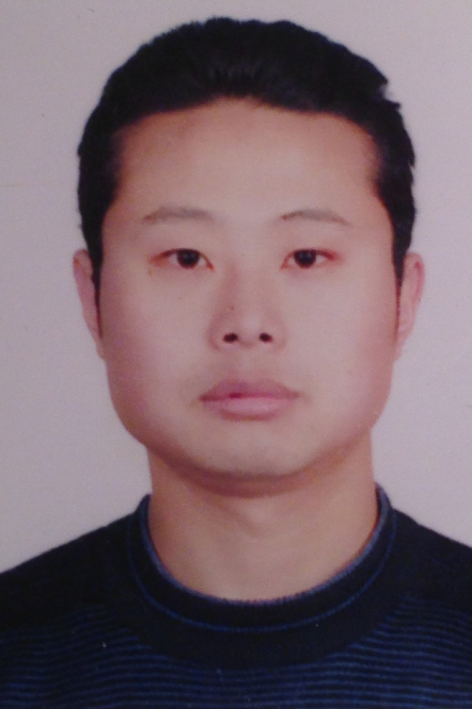
\includegraphics[width=3cm]{myself1}
}
}
}

%\newcommand\BackgroundPic{
%\put(450,550){
%\parbox[t]{\textwidth}{
%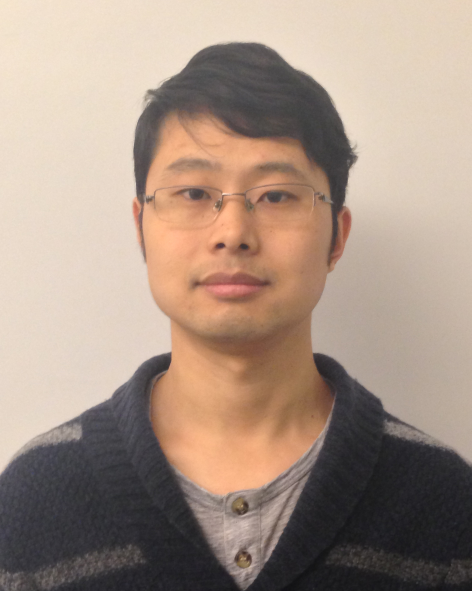
\includegraphics[width=3cm]{myself}
%}
%}
%}

\begin{document}

%----------------------------------------------------------------------------------------
%	EDUCATION SECTION
%----------------------------------------------------------------------------------------

%\begin{textblock}{14}(11,2.1)
%  
\includegraphics[width=4.22cm]{kth}
% \end{textblock}

\AddToShipoutPicture*{\BackgroundPic}

%\rfoot{Kungliga Tekniska högskolan, Brinnellvägen 23, SE-100 44 Stockholm. Tel: +46 (0)70 780 86 42. E-post: Rongzhen.Chen@mse.kth.se}
\begin{rSection}{PERSONAL DETAILS}
 {\bf Name: } \hspace*{14mm} Rongzhen Chen \\
 {\bf Gender: } \hspace*{11mm} Male \\
 {\bf Date of Birth: } August 04, 1983 \\
 {\bf Address: } \hspace*{10mm}  Brinellvägen 23, 100 44 Stockholm, Sweden \\
 {\bf Phone: } \hspace*{14mm}  +46 (0) 70 780 86 42  \\
 {\bf Email: } \hspace*{14mm}  Rongzhen.Chen@mse.kth.se  \\ 
 

 
\end{rSection}

\vspace*{1\baselineskip}

\begin{rSection}{EDUCATION}

{\bf KTH Royal Institute of Technology, Sweden} \hfill { Sept. 2009 -- Sept. 2014 (expected)} \\ 
Department of Materials Science and Engineering \\
Doctor of Philosophy in Multiscale Materials Modelling.

Projects: Implementation of Algorithm within Density Functional Theory (DFT) and DFT-based Simulations in Semiconductor. \\
Courses: Solid State Physics, Nanoscale Materials, Applied Thermodynamics. \\
Supervisors: Prof. Clas Persson and Prof. Börje Johansson. 

{\bf Northeastern University, P. R. China} \hfill { Sept. 2008 -- July 2009} \\ 
College of Information Science and Engineering \\
Research Assistant in Control Theory and Control Engineering.


{\bf Northeastern University, P. R. China} \hfill { Sept. 2006 -- July 2008} \\ 
College of Information Science and Engineering \\
Master of Science in Measuring and Testing Technologies and Instruments.

Courses: Java, Matrix Analysis, Equation of Mathematical Physics. \\
Thesis: ANSYS-based Simulations in the Process of Continuous Casting.

{\bf Shenyang University of Technology, P. R. China} \hfill { Sept. 2002 -- July 2006} \\ 
College of Science \\
Bachelor of Science in Information and Computational Science.

Courses: C language, Data Structure, Numerical Analysis, Physics, Software Engineering. \\
Thesis: Qt-based application: Text Editor.

\end{rSection}

\vspace*{1\baselineskip}

%----------------------------------------------------------------------------------------
%	TECHNICAL STRENGTHS SECTION
%----------------------------------------------------------------------------------------

\begin{rSection}{COMPUTER SKILLS }

\begin{tabular}{ @{} >{\bfseries}l @{\hspace{6ex}} l }
Programming Languages & Fortran, C Language, Java, Python, Bash, SQL \\
Softwares  & Thermo-Calc, Matlab, Eclipse, Github, ANSYS, TotalView, Latex \\
Operating Systems & Windows, Linux, Mac \\
Others & Lapack and Blas Libraries, High Performance Computing, \\
       & Parallel Programming
\end{tabular}

\end{rSection}

\vspace*{1\baselineskip}



%\begin{rSection}{ACTIVITIES AND SOCIETIES}
%$\star$  Developers Week at the Humboldt-Universität zu Berlin in Germany, from Dec. 2nd to Dec. 6th (2013) \\
%$\star$ Visiting in the Group of Prof. Clas Persson at the University of Oslo in Norway, from Apr. to Aug. (2012) \\
%$\star$ Visiting in the Group of Prof. Claudia Ambrosch-Draxl at the University of Leoben in Austria from Oct. to Dec. (2011) \\
%$\star$Introduction to High-Performance Computing, Sweden PDC- Center for High-Performance Computing-Summer School (2011) \\ 
%$\star$ Introduction to High Performance Computing, Finland CSC IT Center for Science Ltd - Summer School (2011) \\
%\end{rSection}



%----------------------------------------------------------------------------------------
%	WORK EXPERIENCE SECTION
%----------------------------------------------------------------------------------------
\begin{rSection}{LANGUAGES}
\textbf{Chinese} (Mother tongue), \textbf{English} (Fluent), \textbf{Swedish} (Beginner, still learning)

\end{rSection}



%\newpage
%\vspace*{1\baselineskip}

\begin{rSection}{research visit}
 
Developers Week for Exciting code at the Humboldt Universität zu Berlin, (02 Dec. -- 06 Dec. 2013) 

The Group of  Prof. Clas Persson at the University of Oslo in Norway (Apr. -- Aug. 2012)

The Group of Prof. Claudia Ambrosch-Draxl at the University of Leoben in Austria (Oct. -- Dec. 2011)

Introduction to High-Performance Computing, Sweden PDC-Summer School (2011) 

Introduction to High Performance Computing, Finland CSC-Summer School (2011)
 
\end{rSection}


\begin{rSection}{ACTIVITIES}


{\bf PhD Student Representative at the Division} (Oct. 2011 -- Present).\\
The duty is to discuss all the issues regarding PhD students' interests.


{\bf Class President} (Sept. 2002 -- July 2006).\\
The duty is to resolve problems for students and report to the department, as well as leading class cabinet meetings and organizing activities and events.
                            
\end{rSection}

\begin{rSection}{AWARDS}
Liaoning Provincial triple A Outstanding Student (2006)\\
Liaoning Provincial Outstanding class cadre (2006)
\end{rSection}






\newpage

%\begin{comment}
 


\begin{rSection}{References}


{\bf Prof. Börje Johansson} \\
Applied Materials Physics \\
Department of Materials Science and Engineering \\
KTH Royal Institute of Technology \\
SE – 100 44 Stockholm, Sweden  \\
Phone: +46 (0) 70 417 54 52 \\
Email: borje.johansson@physics.uu.se \\
  \hspace*{11.5mm}     borjej@kth.se \\
  


{\bf Prof. Clas Persson} \\
Multiscale Materials Modelling \\
Department of Materials Science and Engineering \\
KTH Royal Institute of Technology \\
SE – 100 44 Stockholm, Sweden \\
 -- and -- \\
Department of Physics \\
University of Oslo \\
NO-0316 Oslo, Norway \\
Phone: +46 (0)8-790 8332\\
Email: Clas.Persson@mse.kth.se \\


{\bf Prof. Malin Selleby} \\
Division of Computational Thermodynamics \\
Department of Materials Science and Engineering \\
KTH Royal Institute of Technology \\
SE-100 44 Stockholm, Sweden \\
Phone: +46 (0)8-790 8389  \\
Email: malin@kth.se \\


{\bf Dr. Huahai Mao} \\
Division of Computational Thermodynamics \\
Department of Materials Science and Engineering \\
KTH Royal Institute of Technology \\
SE-100 44 Stockholm, Sweden \\
Phone: +46 (0)8-790 6597 \\
Email: huahai@kth.se \\


\end{rSection}

%\end{comment}


\end{document}
